% DFA for an LR parser
\documentclass{article}
\usepackage{tikz}
\usetikzlibrary{arrows.meta,decorations.pathmorphing,backgrounds,positioning,fit,petri}
\begin{document}
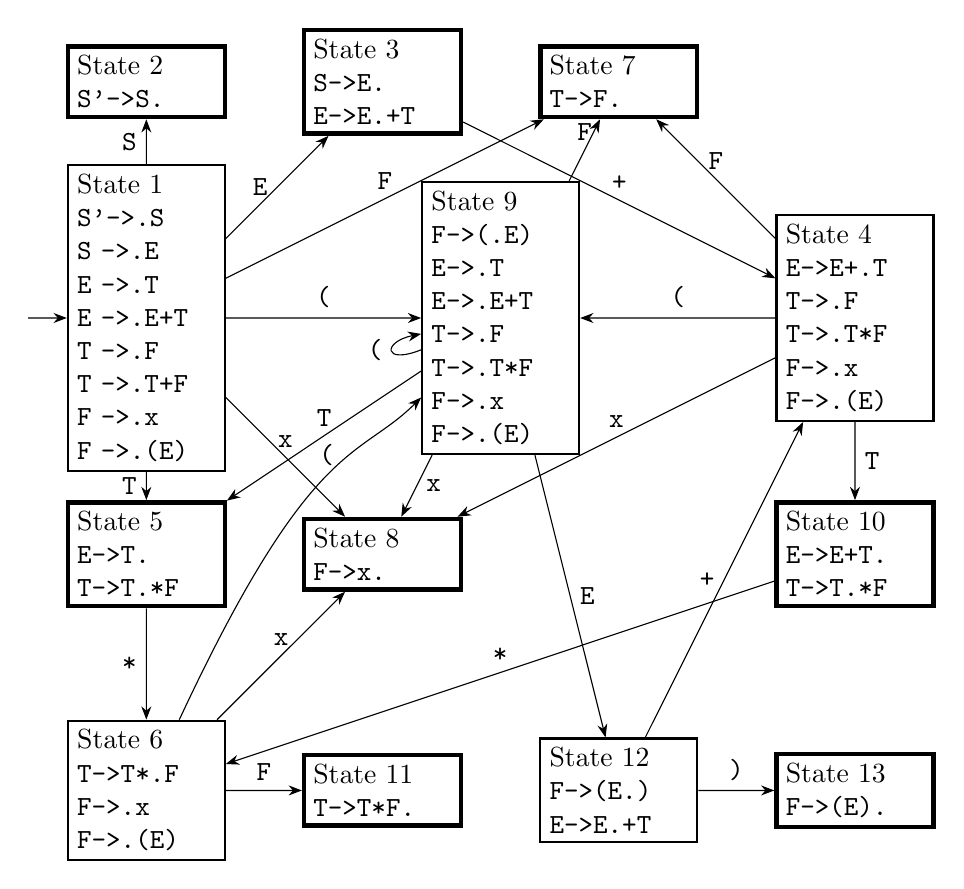
\begin{tikzpicture}[scale=3, >=Stealth,
   state/.style={rectangle, text width=50, thick},
   final/.style={ultra thick}]
   \node (q1) at (1,10) [draw, state] {State 1\\
\texttt{S'->.S}\\
\texttt{S ->.E}\\
\texttt{E ->.T}\\
\texttt{E ->.E+T}\\
\texttt{T ->.F}\\
\texttt{T ->.T+F}\\
\texttt{F ->.x}\\
\texttt{F ->.(E)}};
   \node (q2) at (1, 11) [draw, state, final] {State 2\\
\texttt{S'->S.}};
   \node (q3) at (2, 11) [draw, state, final] {State 3\\
\texttt{S->E.}\\
\texttt{E->E.+T}};
   \node (q4) at (4, 10) [draw, state] {State 4\\
\texttt{E->E+.T}\\
\texttt{T->.F}\\
\texttt{T->.T*F}\\
\texttt{F->.x}\\
\texttt{F->.(E)}};
   \node (q5) at (1, 9) [draw, state, final] {State 5\\
\texttt{E->T.}\\
\texttt{T->T.*F}};
   \node (q6) at (1, 8) [draw, state] {State 6\\
\texttt{T->T*.F}\\
\texttt{F->.x}\\
\texttt{F->.(E)}};
   \node (q7) at (3, 11) [draw, state, final] {State 7\\
\texttt{T->F.}};
   \node (q8) at (2, 9) [draw, state, final] {State 8\\
\texttt{F->x.}};
   \node (q9) at (2.5, 10) [draw, state] {State 9\\
\texttt{F->(.E)}\\
\texttt{E->.T}\\
\texttt{E->.E+T}\\
\texttt{T->.F}\\
\texttt{T->.T*F}\\
\texttt{F->.x}\\
\texttt{F->.(E)}};
   \node (q10) at (4, 9) [draw, state, final] {State 10\\
\texttt{E->E+T.}\\
\texttt{T->T.*F}};
   \node (q11) at (2, 8) [draw, state, final] {State 11\\
\texttt{T->T*F.}};
   \node (q12) at (3, 8) [draw, state] {State 12\\
\texttt{F->(E.)}\\
\texttt{E->E.+T}};
   \node (q13) at (4, 8) [draw, state, final] {State 13\\
\texttt{F->(E).}};

   \draw (0.5,10)[->] -- (q1);
   \draw (q1)[->] -- node[left]{\texttt{S}} (q2);
   \draw (q1)[->] -- node[left]{\texttt{E}} (q3);
   \draw (q1)[->] -- node[left]{\texttt{T}} (q5);
   \draw (q1)[->] -- node[above]{\texttt{F}} (q7);
   \draw (q1)[->] -- node[above]{\texttt{x}} (q8);
   \draw (q1)[->] -- node[above]{\texttt{(}} (q9);
   \draw (q3)[->] -- node[above]{\texttt{+}} (q4);
   \draw (q4)[->] -- node[above]{\texttt{F}} (q7);
   \draw (q4)[->] -- node[above]{\texttt{x}} (q8);
   \draw (q4)[->] -- node[above]{\texttt{(}} (q9);
   \draw (q4)[->] -- node[right]{\texttt{T}} (q10);
   \draw (q5)[->] -- node[left]{\texttt{*}} (q6);
   \draw (q6)[->] -- node[above]{\texttt{x}} (q8);
   \draw (q6)[->] -- node[above]{\texttt{F}} (q11);
   \draw (q6)[->] .. controls (1.7, 9.5) and (1.9,9.4) .. node[above]{\texttt{(}} (q9);
   \draw (q9)[->] -- node[above]{\texttt{T}} (q5);
   \draw (q9)[->] -- node[right]{\texttt{x}} (q8);
   \draw (q9)[->] -- node[above]{\texttt{F}} (q7);
   \draw (q9)[->] .. controls (2, 9.8) and (2,9.9) .. node[left]{\texttt{(}} (q9);
   \draw (q9)[->] -- node[right]{\texttt{E}} (q12);
   \draw (q10)[->] -- node[above]{\texttt{*}} (q6);
   \draw (q12)[->] -- node[above]{\texttt{)}} (q13);
   \draw (q12)[->] -- node[left]{\texttt{+}} (q4);

\end{tikzpicture}
\end{document}
